%TEX root = ../dissertation.tex

\chapter{Pulsarcast}
\label{chapter:pulsarcast}

In this chapter we will introduce and describe our solution. Pulsarcast is a
peer to peer, pub-sub, topic based system focused on reliability, eventual
delivery guarantees and data persistence. We seek this while not fully
compromising the scalability given by the decentralised nature of our
architecture. Looking through our related work it became clear that few fully
decentralised solutions exist that try provide these kind of guarantees. Yet,
if we carefully look at the most popular and widely adopted centralised pub-sub
solutions it is clear that most of them heavily rely and depend upon these same
guarantees. 

We opted for the simpler topic based subscription model given that, in our
view, a well structured and implemented topic based model is more than enough
for a great percentage of our use cases. In the end, we compromise a bit of the
expressiveness of the system in order to avoid bringing more complexity in,
something we believe will pay off.

This chapter is divided as follows, we will start by covering the use case of
our system in section \ref{use-case}, where we will introduce some of our
broader architectural decisions. Next, we will move to section
\ref{data-structures} where we will deep dive into Pulsarcast's data structure
model and how it is distributed across the network. Finally, we will look into
one of the most important parts of our architecture in section
\ref{subscription-management-event-dissemination} where, based on the covered
related work and the taxonomy we defined, we present the algorithms and
mechanisms used for managing the subscriptions and event dissemination.

\section{Use Case}\label{use-case}

Pulsarcast is a fully decentralised solution, as it has been previously
introduced. This means that each node plays a key part in fulfilling the system
purpose, delivering events and ensuring its dissemination. From a broader
perspective Pulsarcast relies on two overlays to fulfil its needs. Kadmelia
DHT, used for a range of purposes from peer discovery, content discovery and to
bootstrap our other overlay, the Pulsarcast overlay. The Pulsarcast overlay is
actually a set of different overlays or, as we call it, dissemination trees.
These trees are on a per topic basis and are the key factor in the way we
disseminate information across our decentralised network. Figure \ref{fig:pulsarcast-overlays} illustrates the multiple overlays in action.

\begin{figure}[hb!]
  \centering
  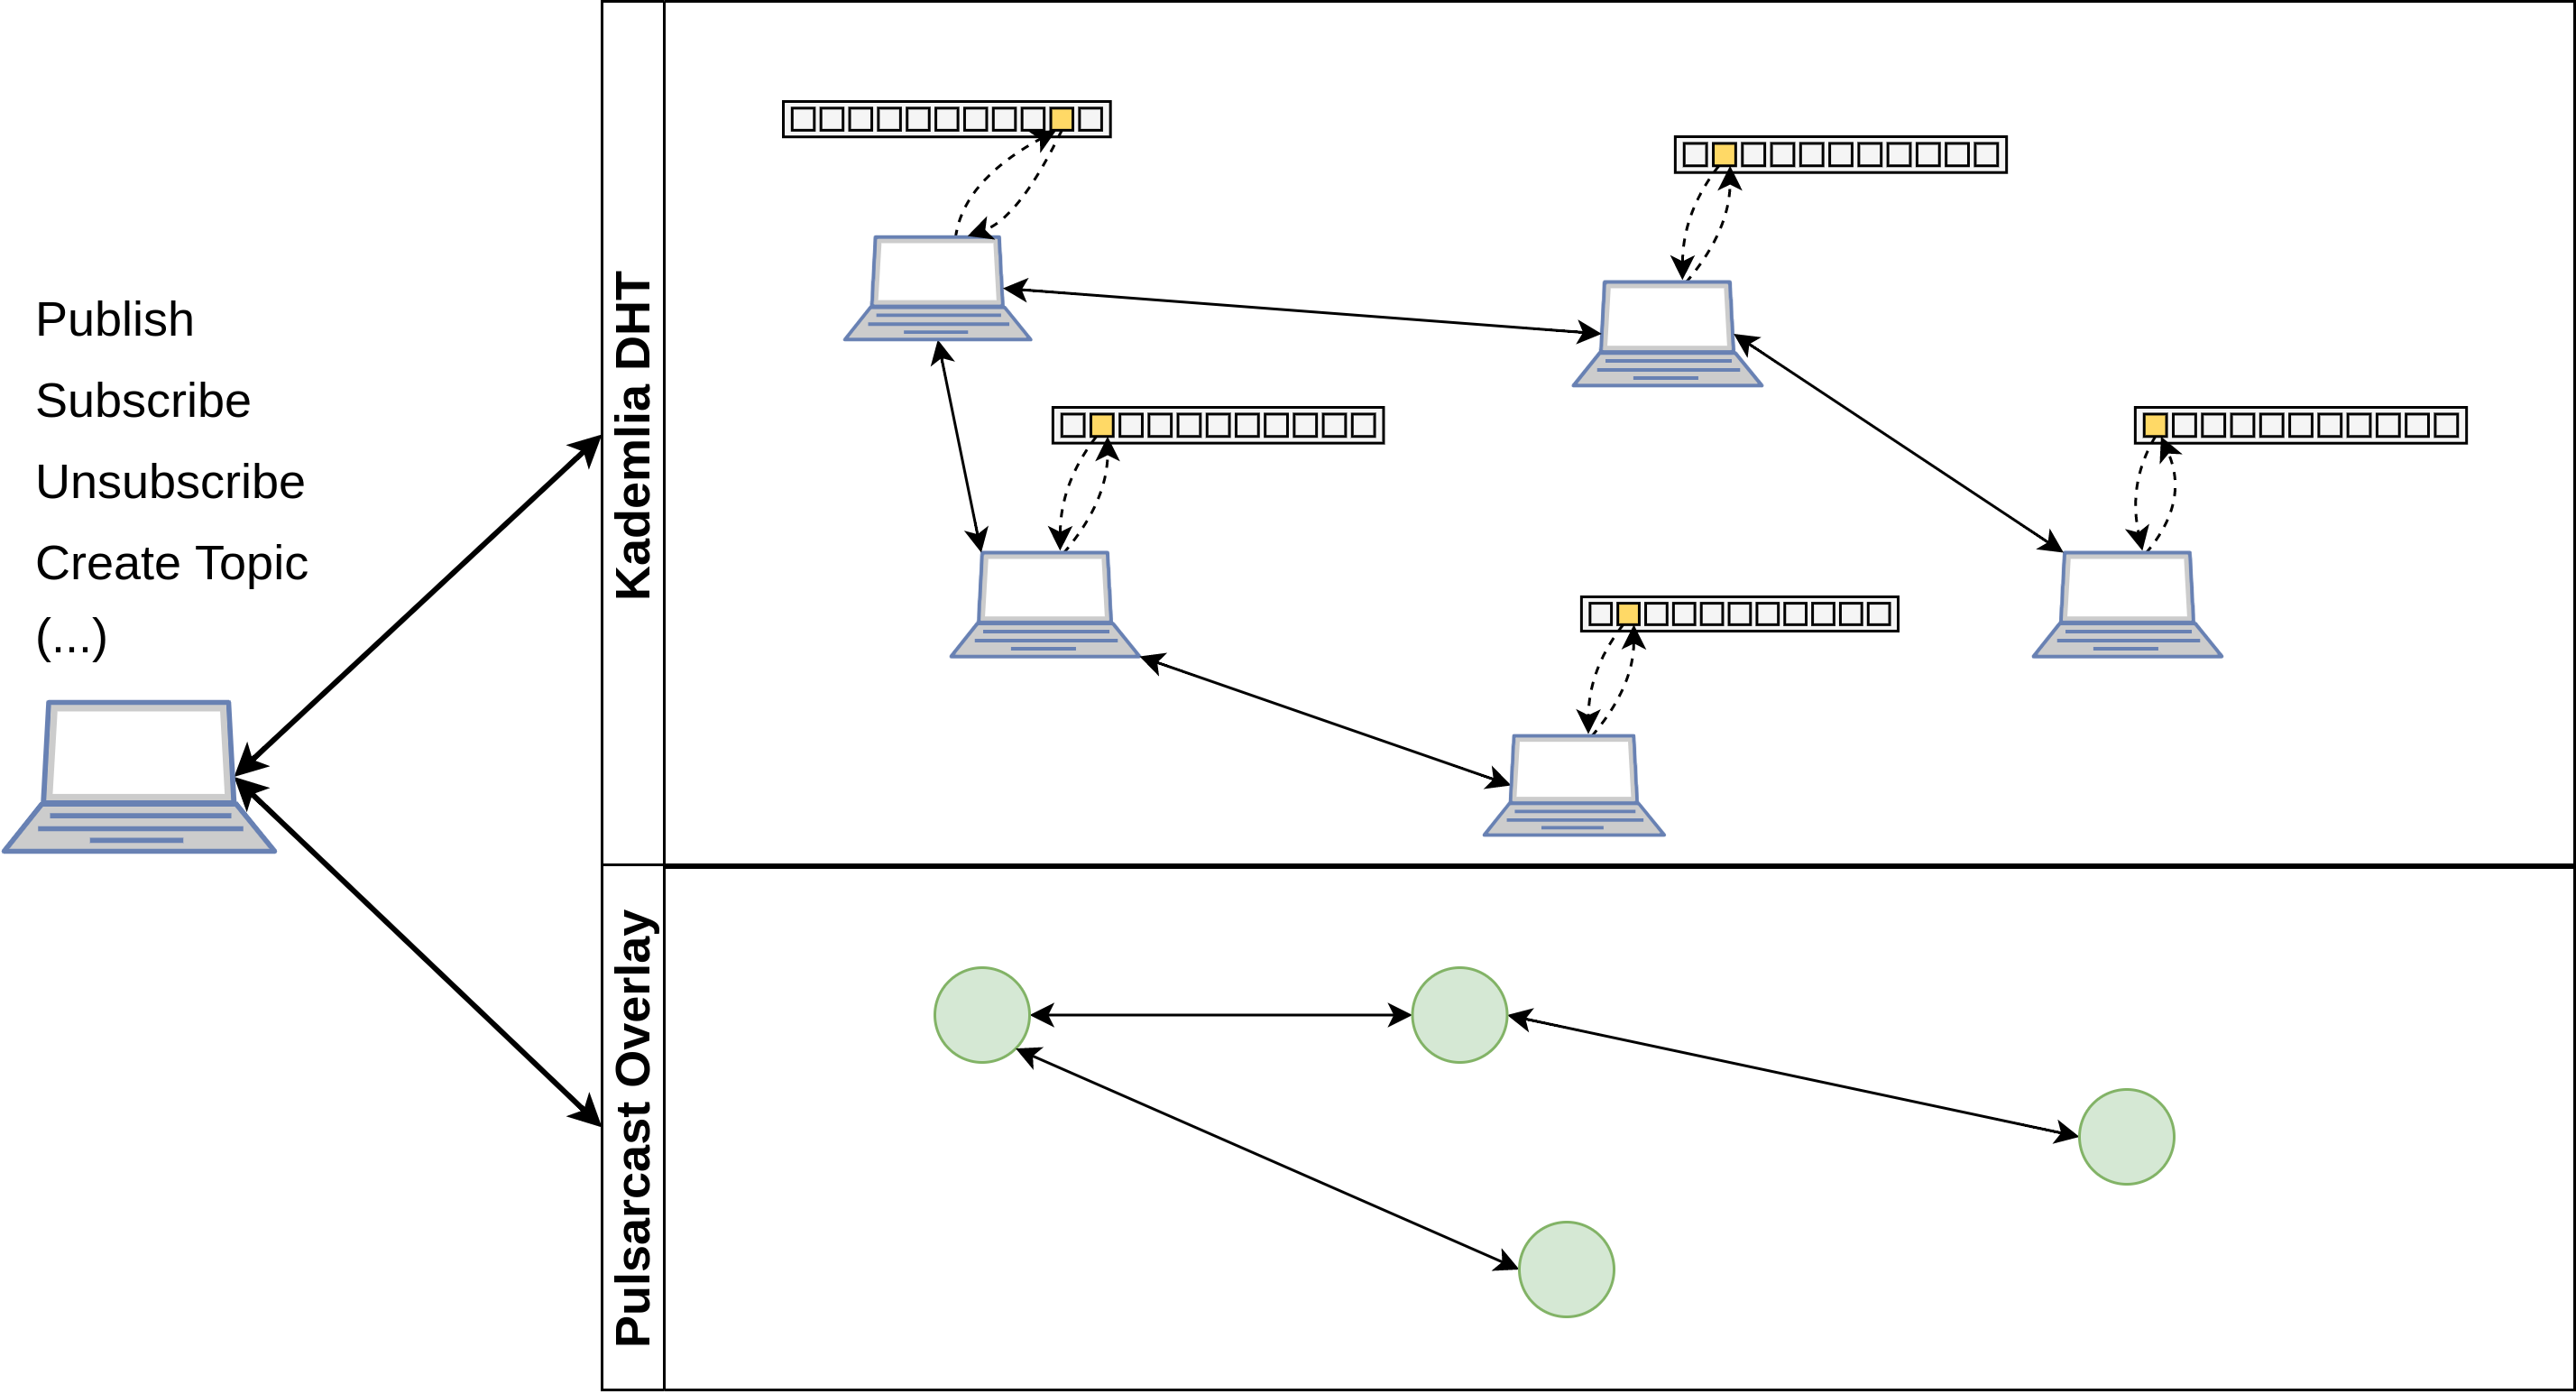
\includegraphics[width=0.95\textwidth]{img/pulsarcast-overlays.png}
  \caption{Representation of the Pulsarcast overlays}
  \label{fig:pulsarcast-overlays}
\end{figure}

The subscription model followed by Pulsarcast is a topic based one, but still
allowing for some expressiveness through the usage of sub-topics to enable more
complex structures. When a peer publishes an event or creates a new topic a set
of the overlays described is used accordingly. For Pulsarcast, both of these
actions, happen to take a similar course. That's because the system views these
pieces of information (or descriptors as we call it) as fairly similar, given
their importance. Figures \ref{fig:pulsarcast-descriptor-creation} and
\ref{fig:pulsarcast-descriptor-query} provide an overview of what flow for
creating this information and for accessing it looks like.

\begin{figure}[hb!]
  \centering
  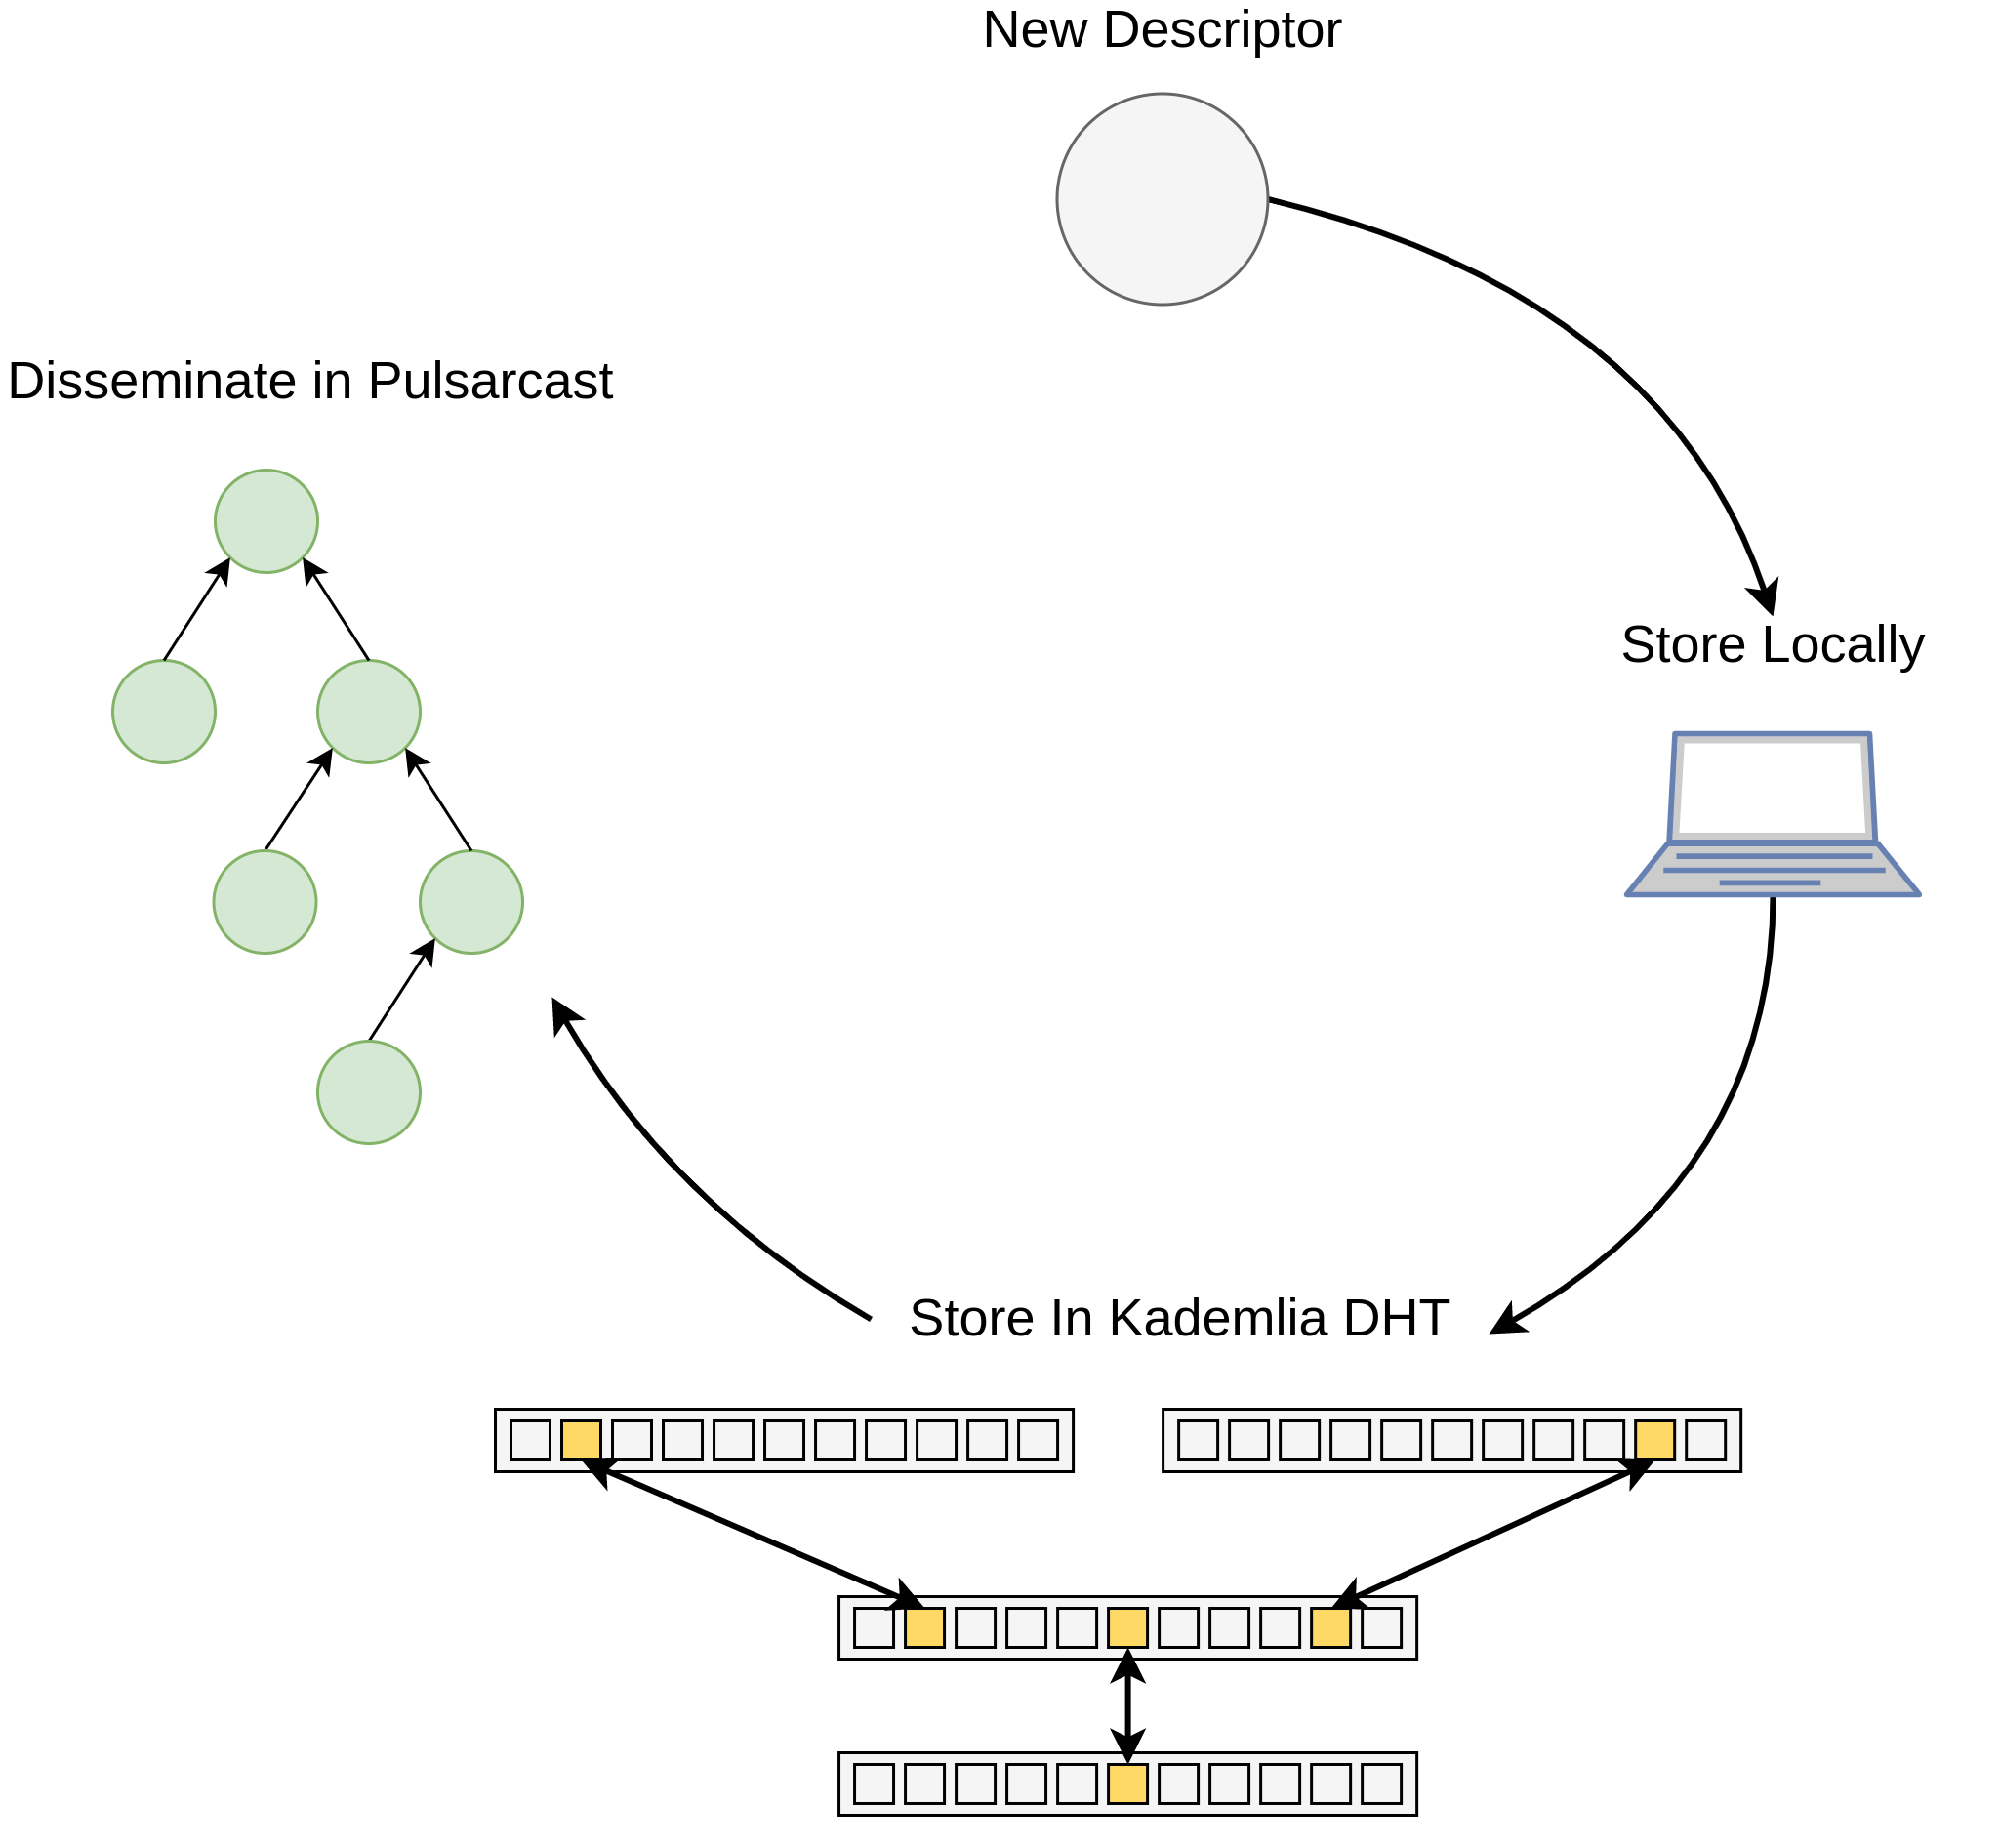
\includegraphics[width=0.7\textwidth]{img/pulsarcast-descriptor-creation.png}
  \caption{Flow for creating a new Topic/Event descriptor}
  \label{fig:pulsarcast-descriptor-creation}
\end{figure}

\begin{figure}[hb!]
  \centering
  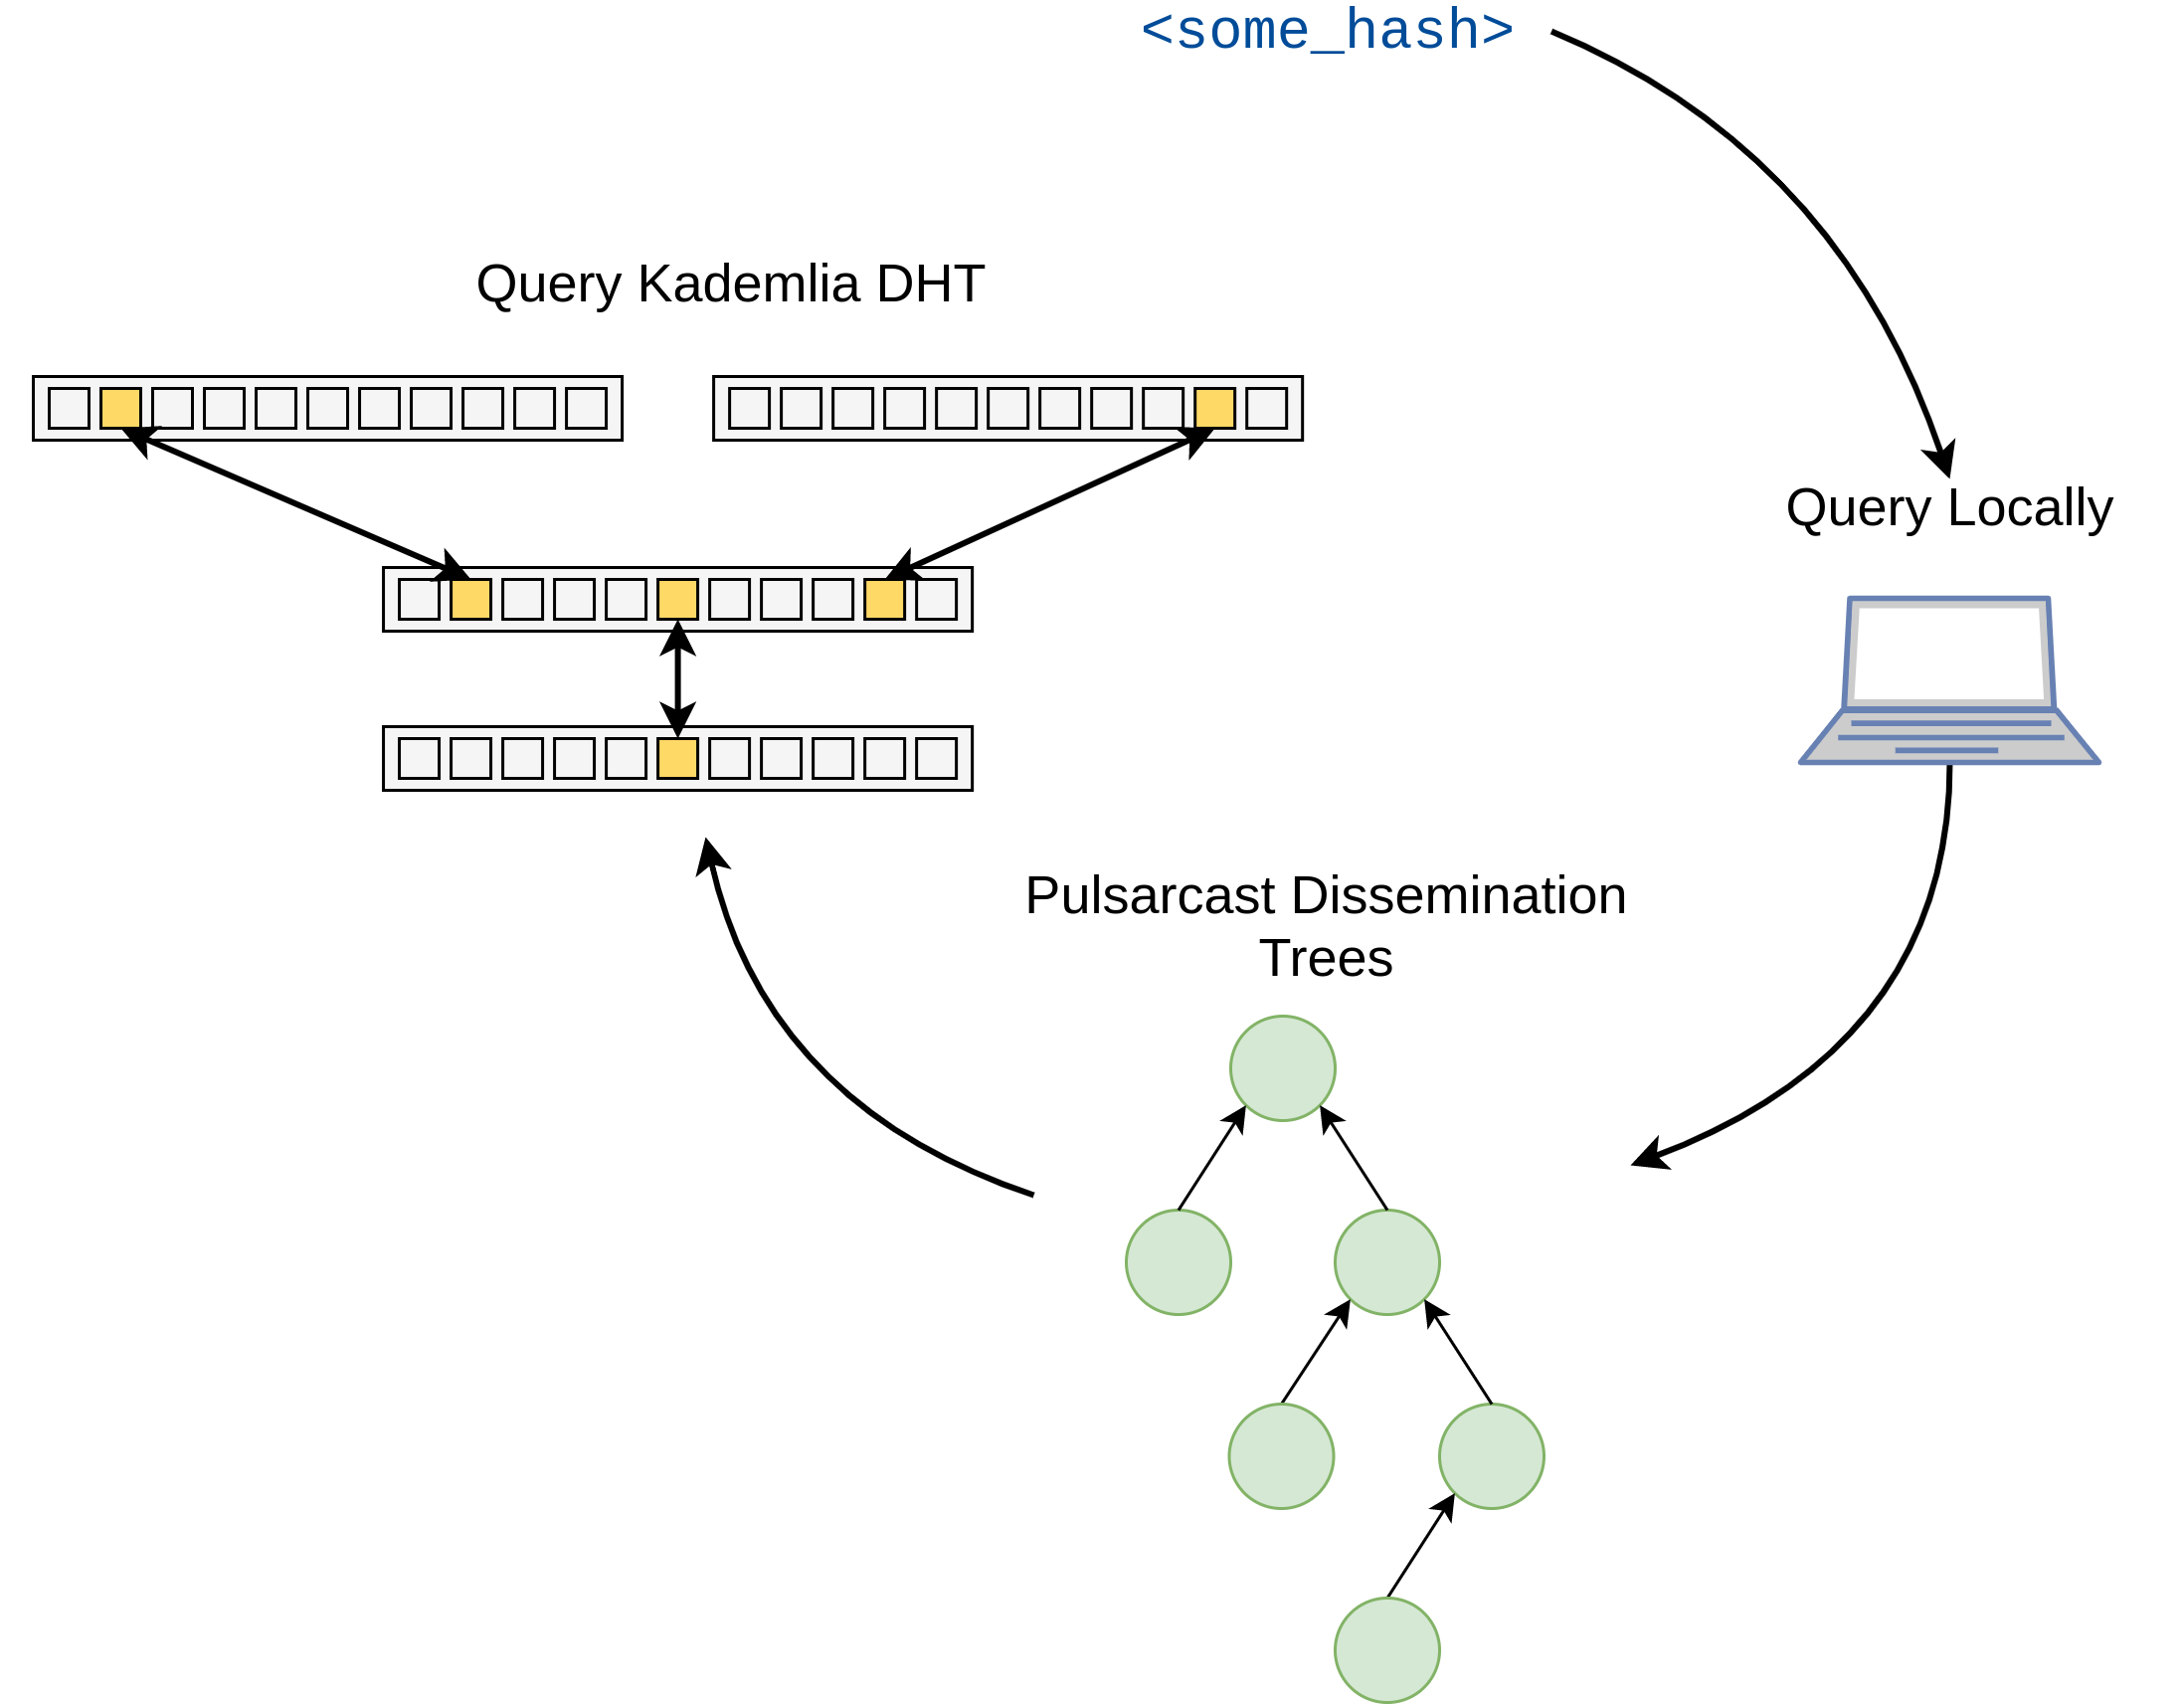
\includegraphics[width=0.7\textwidth]{img/pulsarcast-descriptor-query.png}
  \caption{Flow for querying a Topic/Event descriptor}
  \label{fig:pulsarcast-descriptor-query}
\end{figure}

As Pulsarcast's goal is to give users, and any applications built on top of it,
the reassurance that events reach their destination and that they are able to
rebuild as much of the event or topic history as they see fit, we double down
on our efforts to persist and propagate data. Every topic and event is stored
in the Kadmelia DHT prior to being forwarded through the topic dissemination
trees. This ensures the data is persisted by a set of nodes (that might even be
extraneous to the topic at hand) and anyone is later able to fetch the data
using only the DHT if they want to. Afterwards, we forward the data through the
appropriate dissemination trees previously built (we'll cover tis process in
section TODO). Currently, every node participating in the data transmission through
the dissemination tree stores it indefinitely, although it is something due to
be changed in a later revision of our protocol. On the other hand, when someone
wants to fetch a piece of data (a topic or an event) it starts by performing a
local search in the system, it might have been something that the node as ran
through when forwarding events across their dissemination trees. If this fails
though, a query to the DHT is in order.

\section{Data Structures}\label{data-structures}

Pulsarcast has a set of two very important data structures to which we refer to
as event and topic descriptors. To help us represent this data we rely on a
concept already introduced in our related work, the Merkle DAG.

All of our data structures are immutable, content addressable and linked
together to form a Direct Acyclic Graph. Events link both to their respective
topic descriptor and a past event in that topic. Topics on the other hand, link
to their sub-topics (if any) and a previous version of themselves. Figure
\ref{fig:pulsarcast-dag} provides a broader picture of how it all fits
together. Immutability and content-addressability give us verifiability and,
consequently, the assurance that the state of our distributed system is the
same no matter where we're accessing it from or who's viewing it. It also
allows us to build a notion of history which, if you think about it, plays nice
into a pub-sub scenario. Through these links and the mechanisms described in
the previous section, users and applications are free to rebuild their topic
and event history to any point they wish. Be that because they were not part of
the network at the time or because they missed out due to some system or
network failure, acting as a NACK (not acknowledged) for relevant events.

\begin{figure}[hb!]
  \centering
  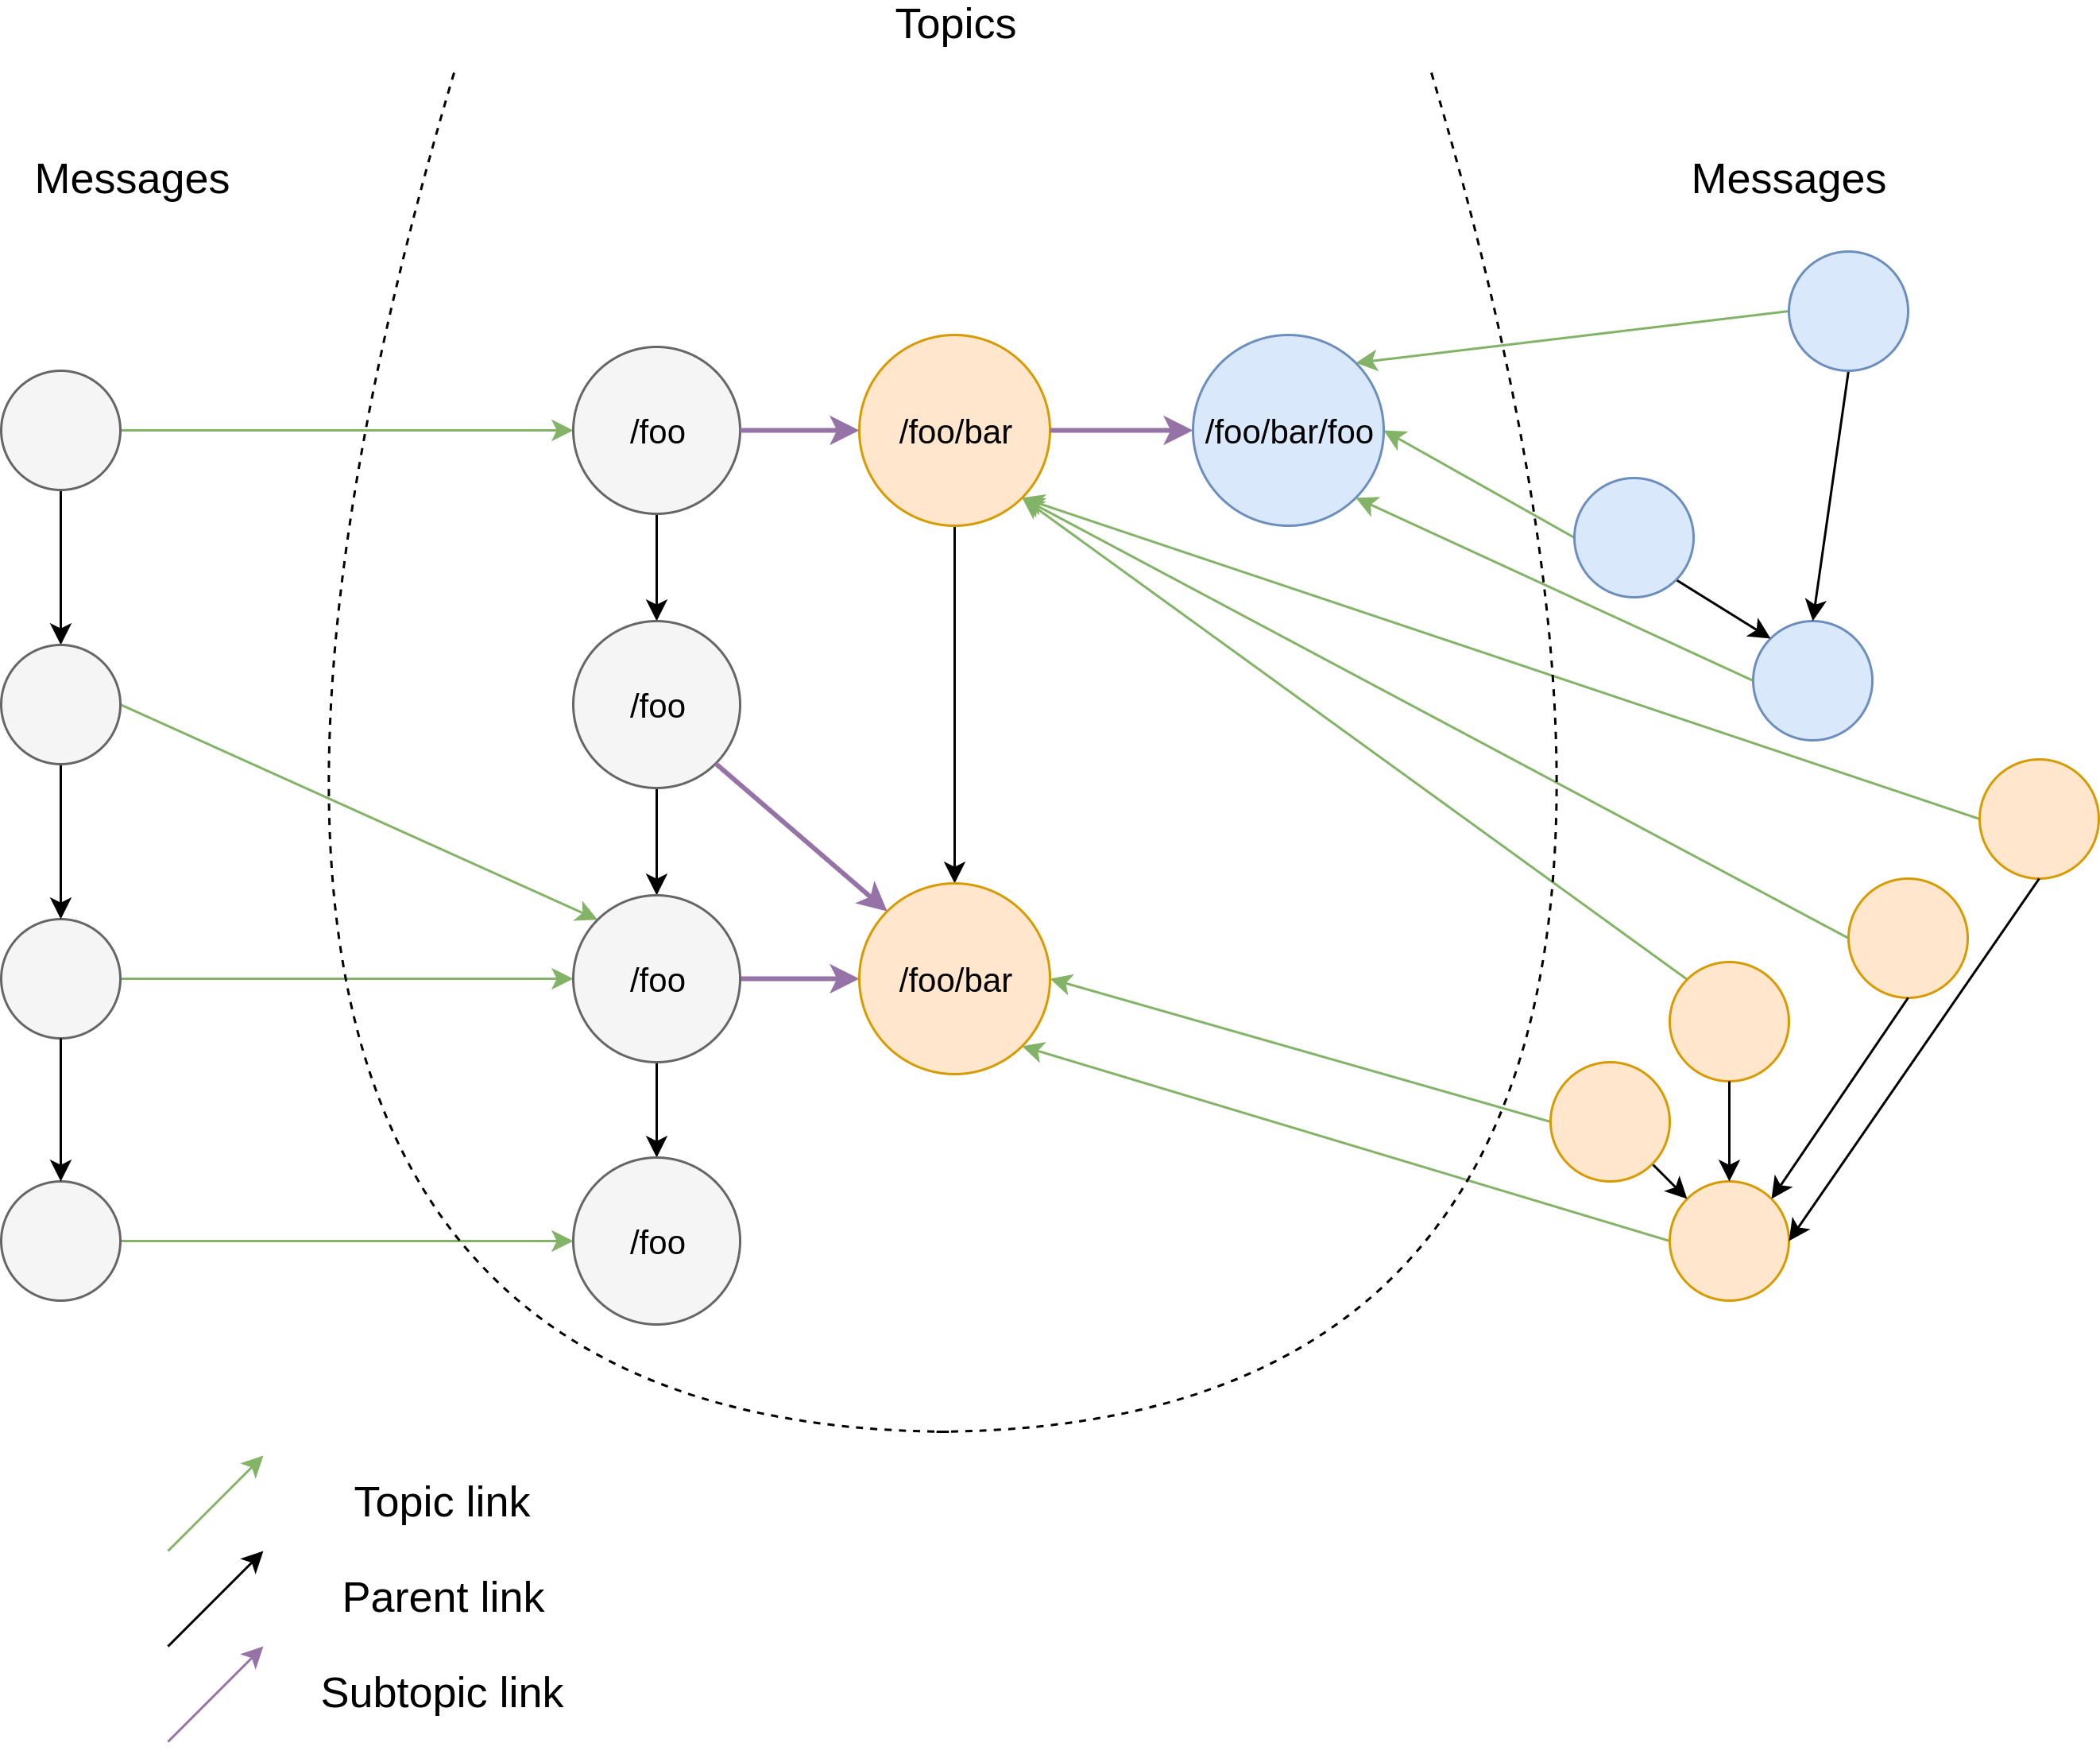
\includegraphics[width=0.95\textwidth]{img/pulsarcast-dag.png}
  \caption{Representation of the Pulsarcast DAG}
  \label{fig:pulsarcast-dag}
\end{figure}

Each of the descriptors contain a set of relevant metadata as well as the
actual information that they refer to. The following JSON like representations
\ref{topic-descriptor} and \ref{event-descriptor} provide an accurate
description of the schema and format of our data structures. We will cover
however some of the properties.

Parent links in the event descriptor serve as a reference to previous events in
the topic tree. A Pulsarcast node that has just received an event can, through
its parent link, know a previous event of this same topic and act on it
accordingly (fetch it or not). Depending on the type of topic we have at hand
(something we will cover further in this document) this parent link can have
different meanings and relevance.

As for the parent links in the topic descriptor, these act as a reference to a
previous version of this same topic. Keep in mind that data in Pulsarcast is
immutable, as such, one cannot update content that has already been published
and disseminated. We can however create a new reference of it and link to what
we consider to be a previous version. This is the exact use case for the parent
links in the topic descriptor, to act as a link to previous versions of this
same topic. Possible changes to the topic descriptor can encompass changes to
the topic metadata for example, or additions of new sub-topics.

In topic descriptors, sub-topic links are indexed under a \emph{\#} key.
Commonly, these are indexed by name, but it is not mandatory, it is actually up
to the topic and consequently its owner to choose accordingly.  There is no
limit to how many sub-topics a topic can have. One really important note though is that every topic actually comes with a default meta topic as a sub topic. The idea is for this meta topic to be used to disseminate changes for the original topic descriptor, something we will cover in section \ref{subscription-management-event-dissemination}.

Both descriptors have an author field that is self descriptive, essentially
meaning the peer responsible for creating and, in the case of the topic,
maintaining this descriptor. The topic descriptor however has an extra field
which is the publisher field. This is because the producer of the content
(author) and the peer responsible for actually pushing this into the Pulsarcast
dissemination trees (publisher) might not actually be the same peer.

\noindent\begin{minipage}{\textwidth}
\vspace{8pt}
\begin{lstlisting}[language=JSON,caption={Topic descriptor schema in a JSON based format},label={topic-descriptor},captionpos=b]
{
  "name": <string>,
  "author": <peer-id>,
  "parent": {                     //The parent link for this topic
    "/": <topic-id>
  },
  "#": {                          //Sub topic links
		meta: {												//Meta topic
			"/": "zdpuAkx9dPaPve3H9ezrtSipCSUhBCGt53EENDv8PrfZNmRnk"
		},
    <topic-name>: {
      "/": <topic-id>
    },
    ...
  },
  "metadata": {
    "created": <date-iso-8601>,
    "protocolVersion": <string>,  //Pulsarcast protocol version
    "allowedPublishers": {        //If enabled, whitelist of allowed publishers
      "enabled": <boolean>,
      "peers": [ <peer-id> ]
    },
    "requestToPublish": {         //Enable request to publish
      "enabled": <boolean>,
      "peers": [ <peer-id> ]      //Optional whitelist able to request
    },
    "eventLinking": <string>,     //One of: LAST_SEEN, CUSTOM
  }
}
\end{lstlisting}
\vspace{8pt}
\end{minipage}

Metadata for the event descriptor is quite simple. It includes a creation
timestamp in ISO8601 format and the version of the protocol at the time the
event was published. Remember, these are content addressable immutable data
structures, as such the info we provide in these metadata fields will be
persistent and verifiable, something we take advantage of. On the other hand
the topic descriptor is a bit more complex. Besides the timestamp and version,
it includes further configuration options that tell us how event dissemination
and event linking will be handled for all of the topic, something we will cover
in section \ref{subscription-management-event-dissemination}.

A key objective for these data structures and, specifically, to the metadata
design has been for it to be easily extensible. The protocol version aids us
with this, easily conveying any kind of breaking changes. Examples of fields
and properties that could be added in the future include things such as author
and publisher signatures, so that peers could verify the authenticity of all
the content.

\noindent\begin{minipage}{\textwidth}
\vspace{8pt}
\begin{lstlisting}[language=JSON,caption={Event descriptor schema in a JSON based format},label={event-descriptor},captionpos=b]
{
  "name": <string>,
  "publisher": <peer-id>,         //Peer who published the event
  "author": <peer-id>,            //Author of the event
  "parent": {                     //The parent link for this event
    "/": <topic-id>
  },
  "topic": {
    "/": <topic-id>
  },
  "payload": <binary-data>
  "metadata": {
    "created": <date-iso-8601>,
    "protocolVersion": <string>,  //Pulsarcast protocol version
  }
}
\end{lstlisting}
\vspace{8pt}
\end{minipage}

The data in Pulsarcast however is distributed, as illustrated by figure \ref{fig:pulsarcast-local-vs-distributed-state}, which means we have to deal with
an extra layer of complexity in our system. We again tackle this with the way
our data is represented, the Merkle DAG. The fact that all the data is
addressed based on its content means that the representation and indexing done
at each node is the same we do system wide. Descriptors are persisted using the
Kadmelia DHT and disseminated through the Pulsarcast overlay, with each node
then keeping this state locally. This allows us to abstract state at each node
in a manner where you can refer to the same piece of data in the same way and
expect the same representation and result, weather you're looking locally or
system wide.

\begin{figure}[hb!]
  \centering
  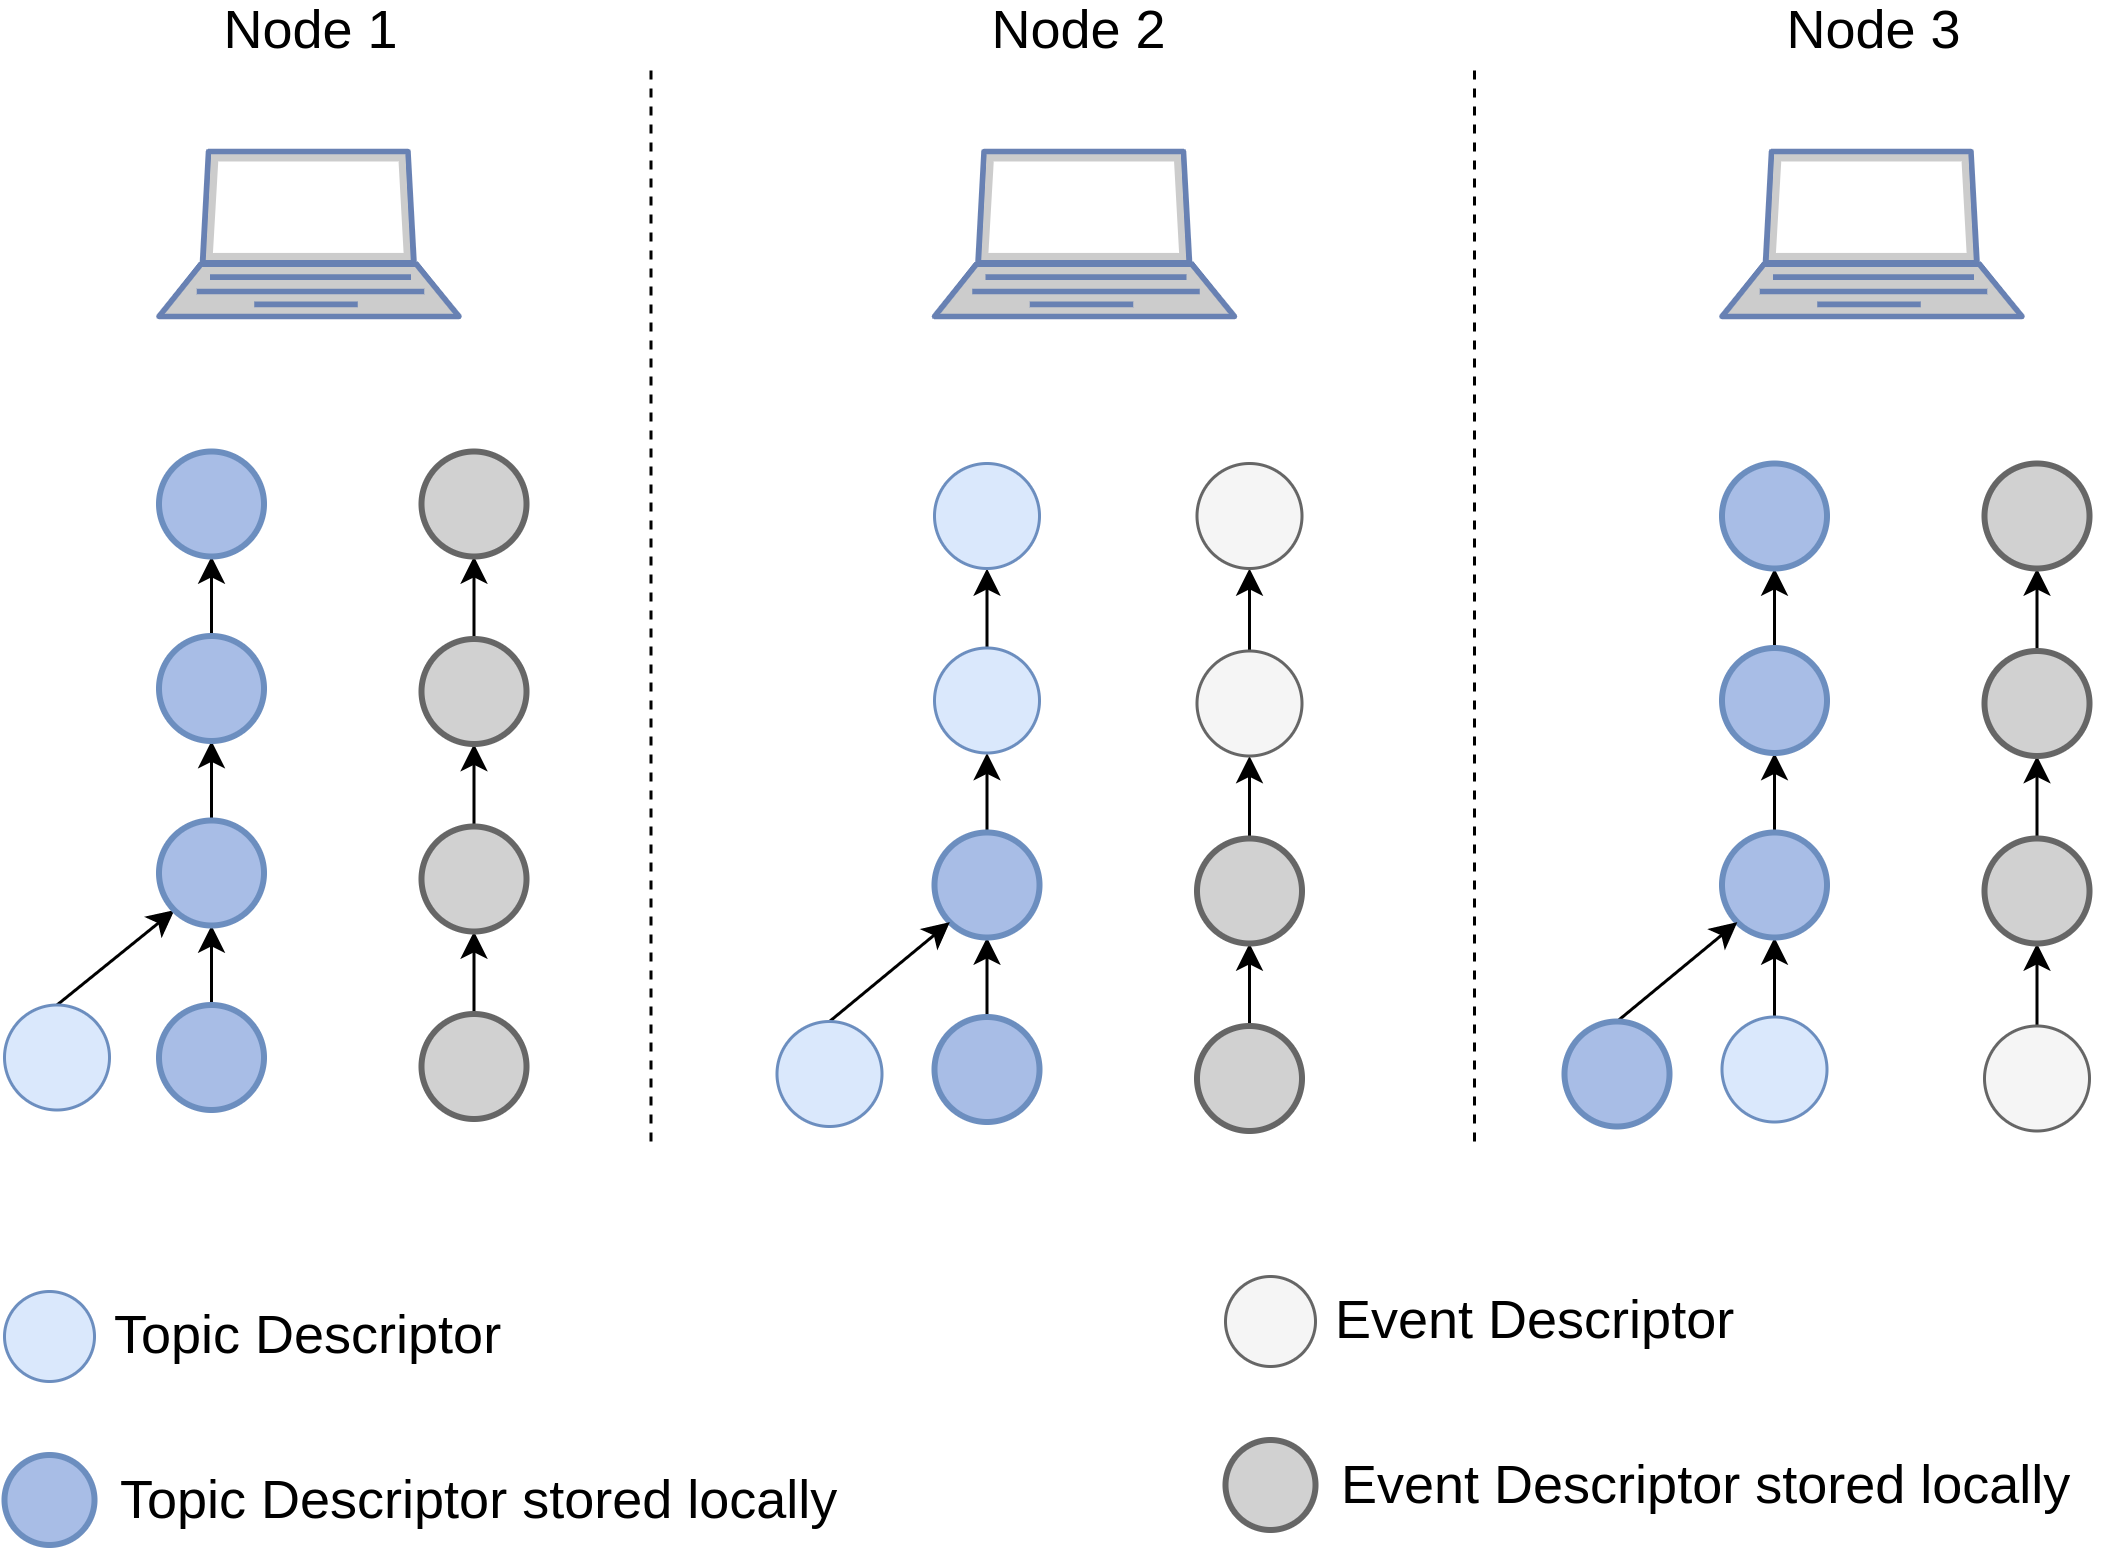
\includegraphics[width=0.8\textwidth]{img/pulsarcast-local-vs-distributed-state.png}
  \caption{Overview of how state is kept across the network}
  \label{fig:pulsarcast-local-vs-distributed-state}
\end{figure}

\section{Subscription Management and Event Dissemination}\label{subscription-management-event-dissemination}

In Pulsarcast, both the subscription management and the event dissemination lie
on top of the multiple overlays built on a per topic basis or, as we call it,
the dissemination trees. These trees represent the path traversed by the events
in order to reach the necessary subscribers, so, in the end, these end up being
the actual representation of both subscriptions and dissemination paths. In
order to better understand them we will start by understanding how the system
handles the creation of topics, new subscriptions, followed by how events are
propagated (with a detailed view of the algorithms used). We will see some of
the configurations the topic descriptor allows for that will change the way
events are propagated and published. Finally we will run through the messages
sent by each node in order to perform these operations, a key part in our
distributed system.

Before we can speak about a new subscription a topic must already exist. As we have detailed previously, a node creates a topic descriptor and stores it in the Kadmelia DHT, making it available to the whole network. From this point on, this node will act as the root node in this newly created topic dissemination tree. When a node wants to subscribe to this topic it starts by fetching it from the Kademlia DHT

TODO
\begin{itemize}
\item Árvores de disseminação
\item Event linking (last seen vs custom)
\item Request to publish
\item Allowed publishers
\item Uso da DHT
\item Algoritmos em detalhe
\item Disseminação de eventos
\end{itemize}

TODO

\begin{figure}[hb!]
  \centering
  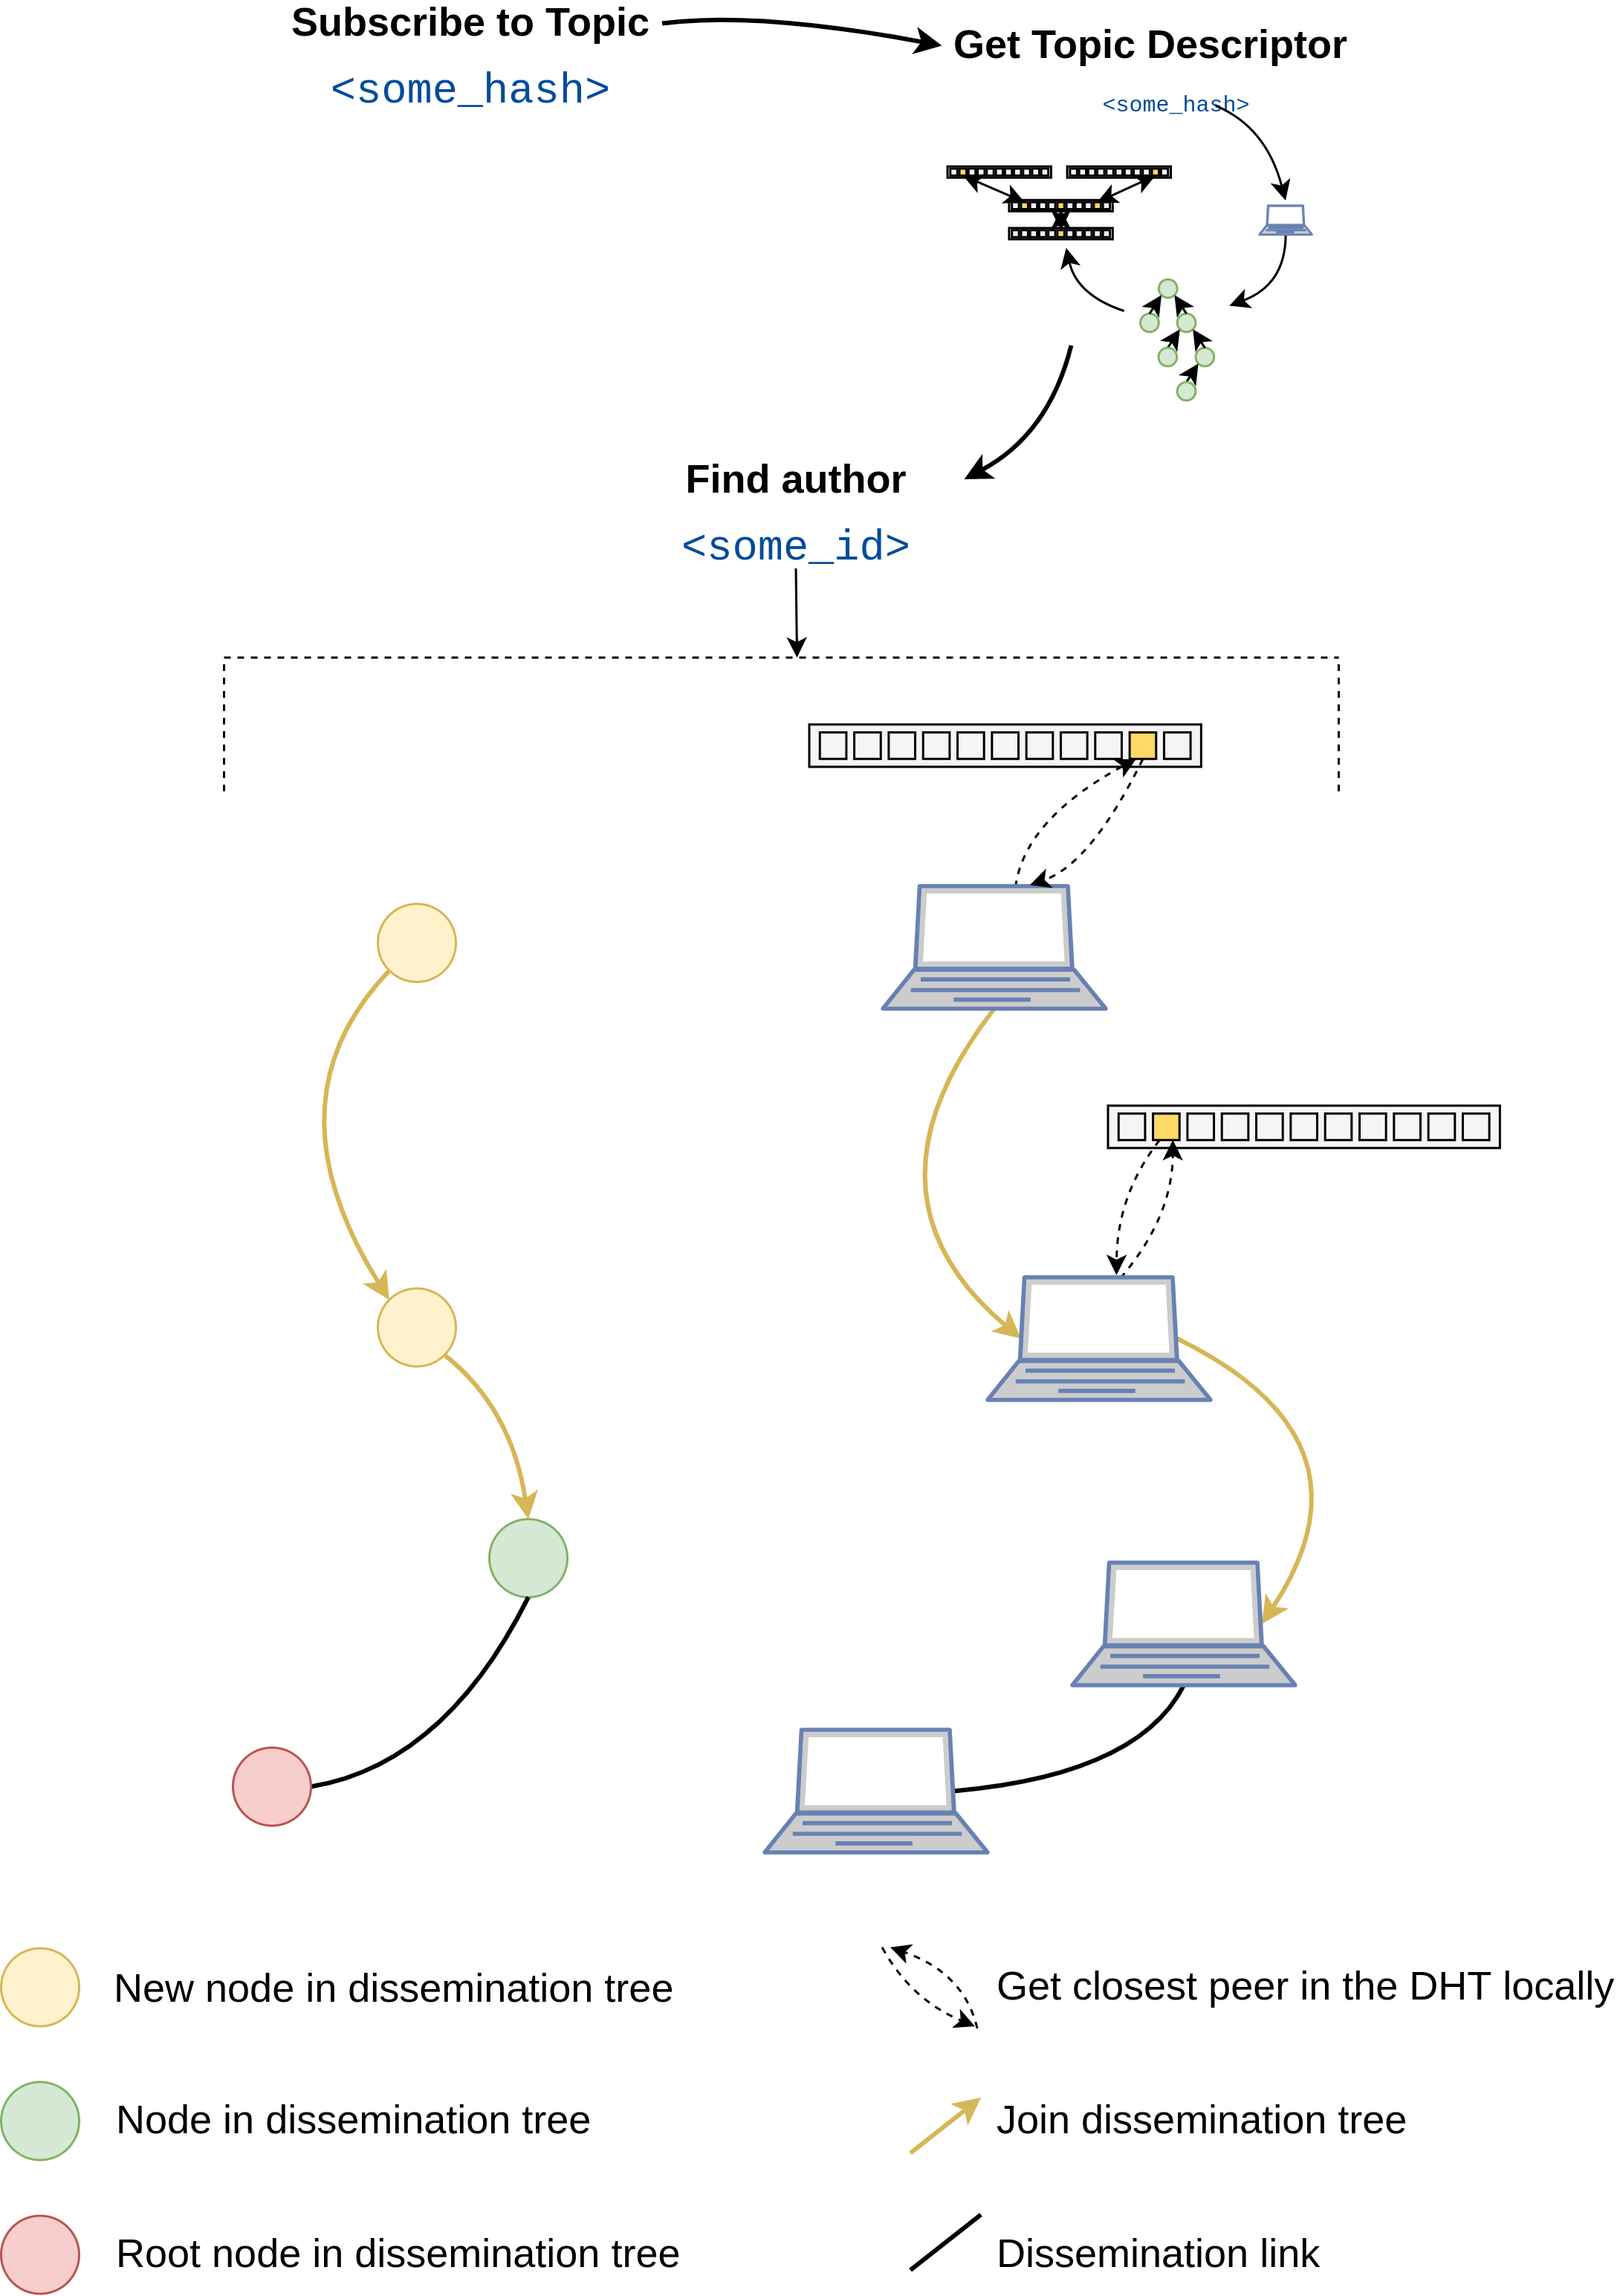
\includegraphics[width=0.8\textwidth]{img/pulsarcast-subscription-flow.png}
  \caption{Overview of the flow for creating a new subscription}
  \label{fig:pulsarcast-subscription-flow}
\end{figure}

TODO

\begin{figure}[hb!]
  \centering
  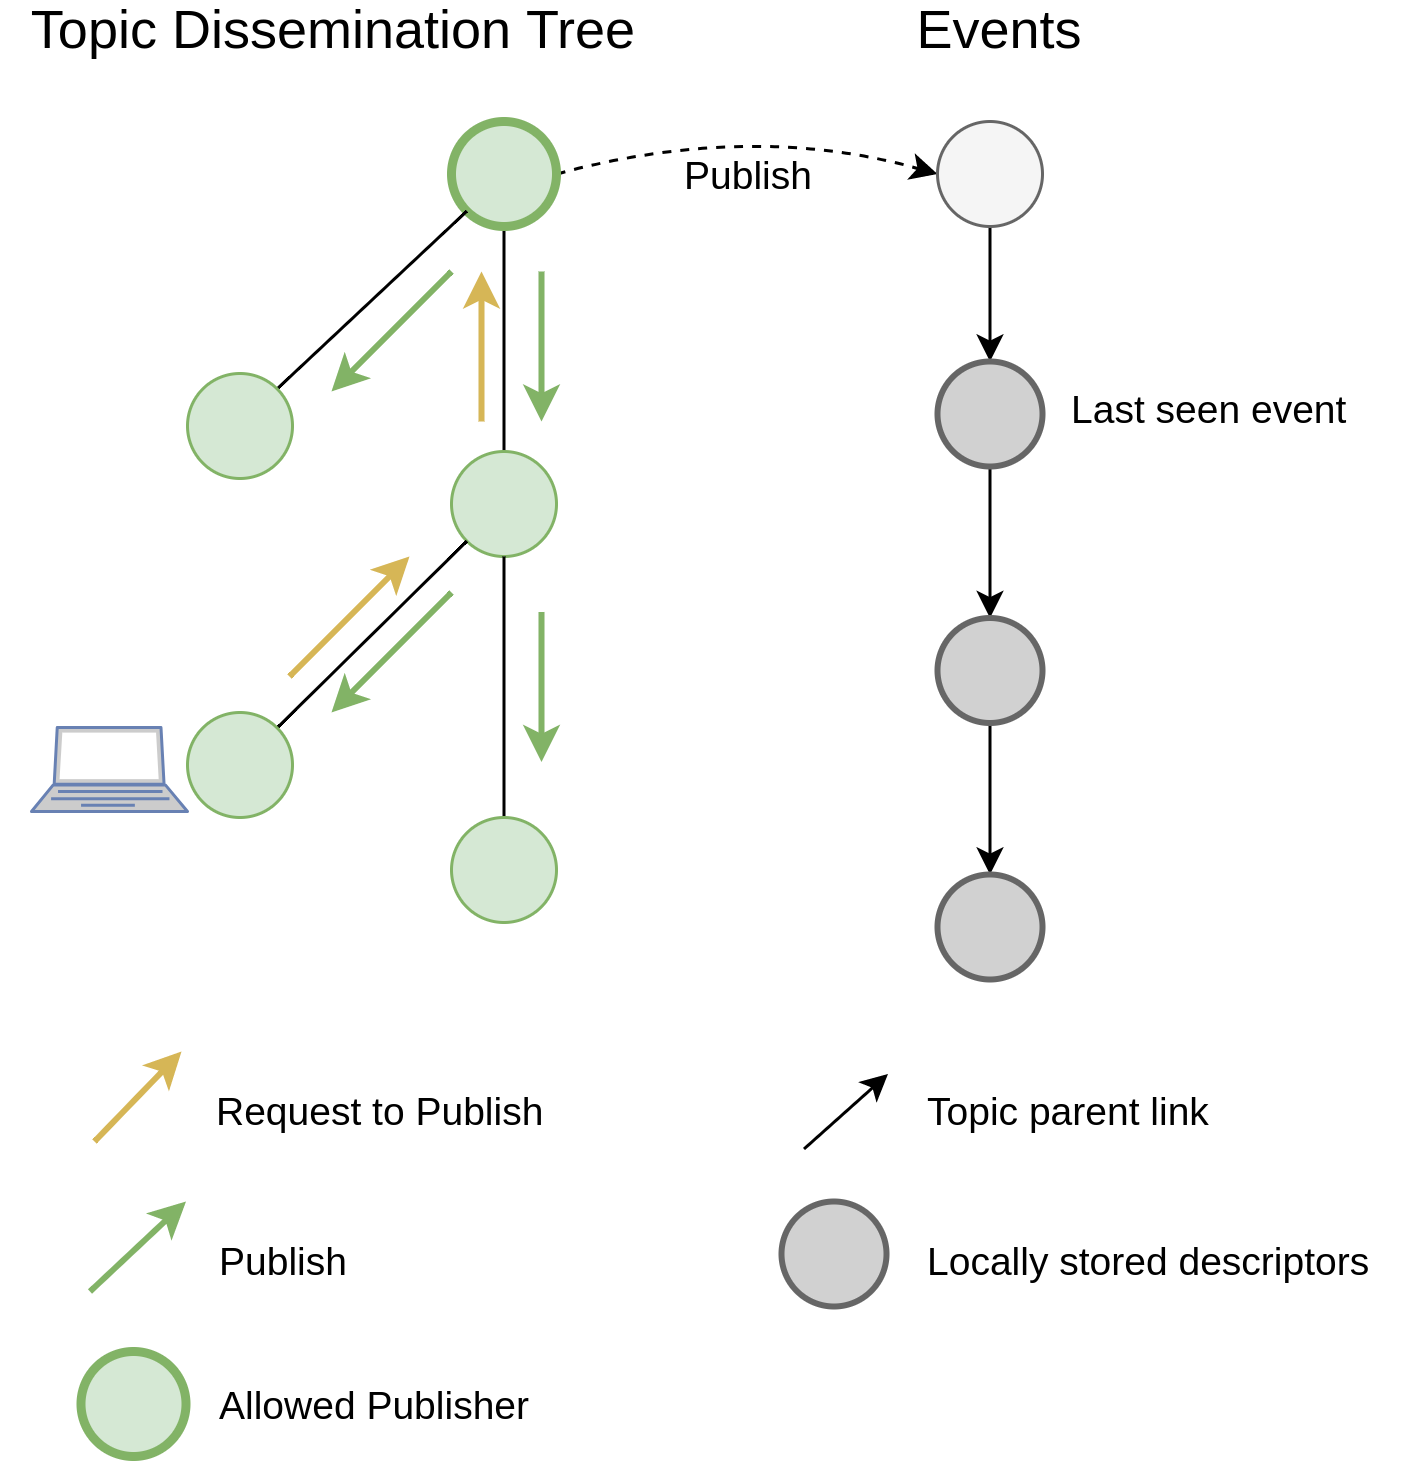
\includegraphics[width=0.6\textwidth]{img/pulsarcast-publish-order-guarantee.png}
  \caption{Event dissemination mechanism for a topic with a order guarantee configuration}
  \label{fig:pulsarcast-publish-order-guarantee}
\end{figure}

TODO

\begin{figure}[hb!]
  \centering
  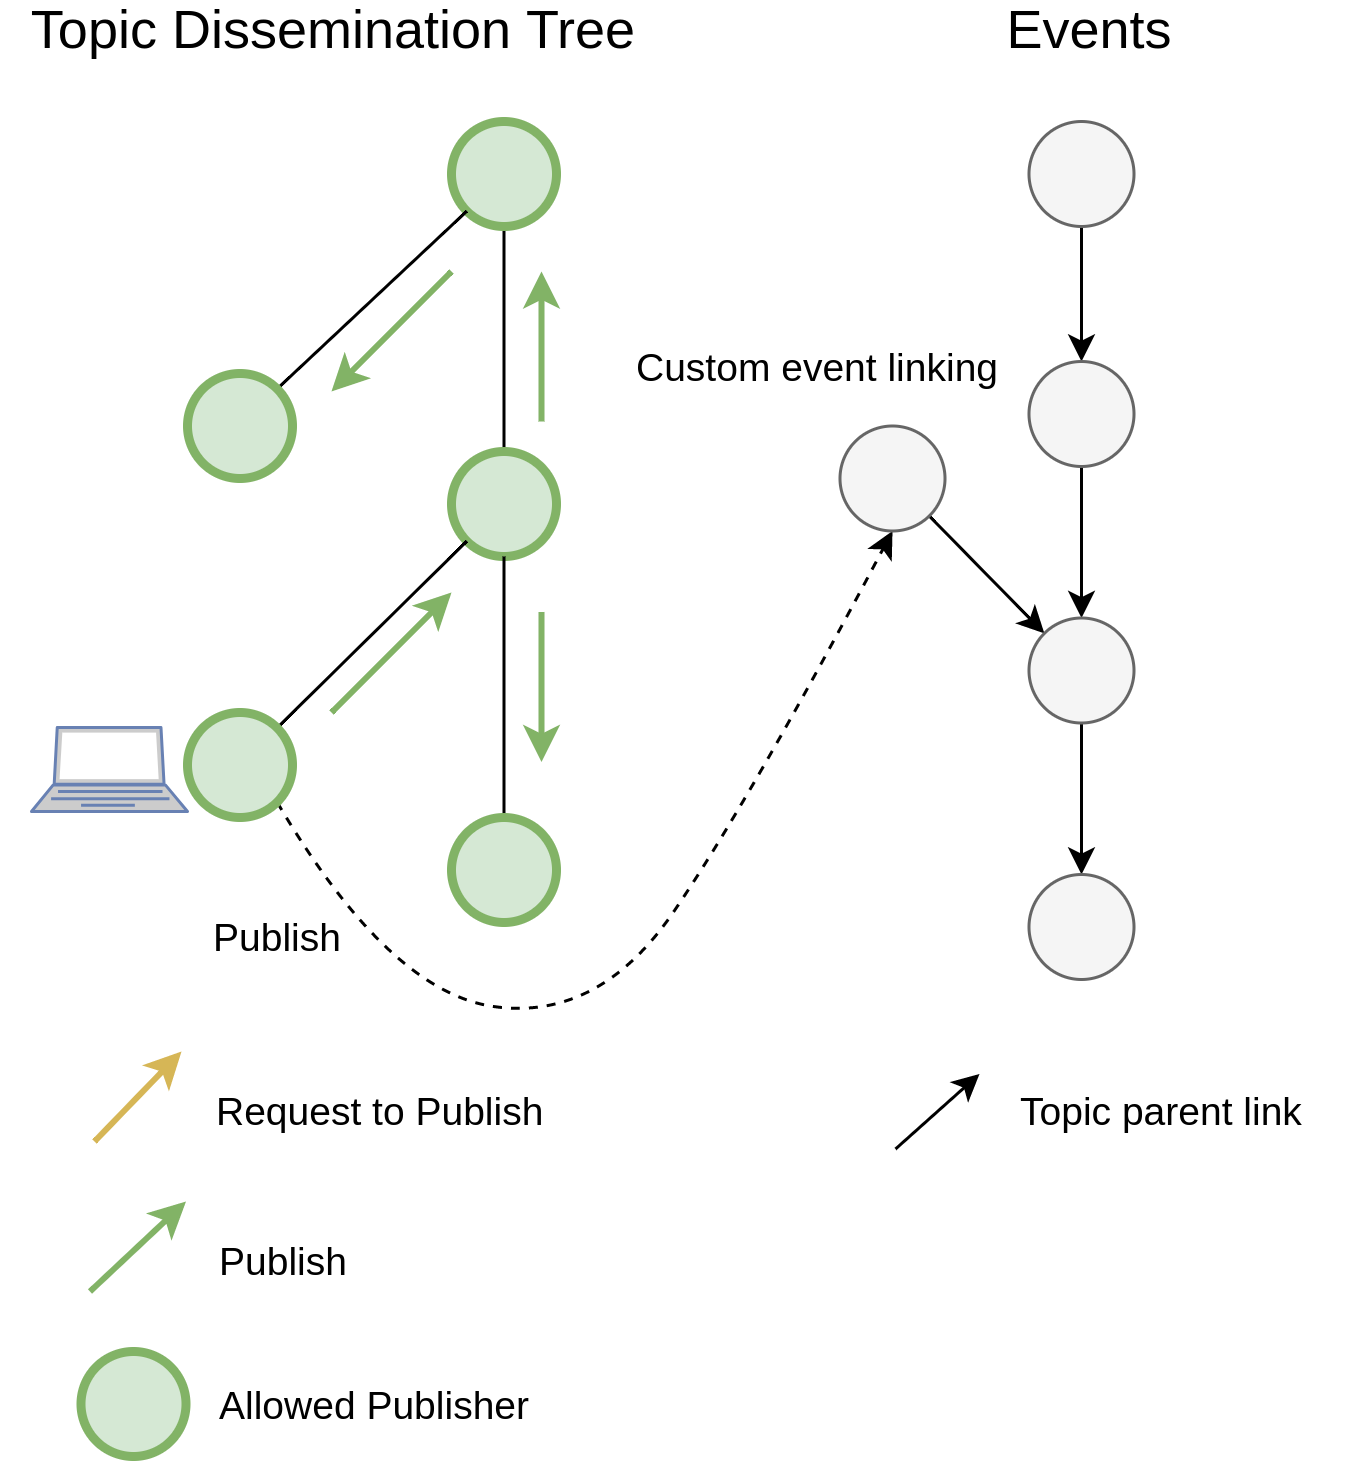
\includegraphics[width=0.6\textwidth]{img/pulsarcast-publish-custom.png}
  \caption{Event dissemination mechanism for a topic with custom event linking and global publishers allowed}
  \label{fig:pulsarcast-publish-custom}
\end{figure}

TODO


\SetKwProg{Fn}{Function}{}{}

\begin{algorithm}[H]
  \SetAlgoLined
  \Fn{CreateTopic(newTopic)}{
  	\KwIn{$newTopic=$ data for new topic creation}
		\BlankLine
  	\Begin{
			$parent \leftarrow newTopic.parent$\;
  	  \eIf(\tcp*[r]{Check if the topic has a parent link}){$parent == null$}{
				$metaTopic \leftarrow CreateMetaTopicDescriptor(newTopic)$\;
  	  }{
				$metaTopic \leftarrow parent.subTopics.meta$\;
			}
			$topicData \leftarrow CreateTopicDescriptor(newTopic, metaTopic)$\;
			$Subscribe(metaTopic)$\;
			$Subscribe(topicData)$\;
			$StoreInDHT(metaTopic)$\;
			$StoreInDHT(topicData)$\;
			$Publish(metaTopic, topicData)$\tcp*[r]{Publish the new topic in the meta topic}\
  	}
	}
  \caption{Create a new topic}
\end{algorithm}

TODO

\begin{algorithm}[H]
  \SetAlgoLined
  \Fn{ReceivedJoin(fromNodeId, topicId)}{
  	\KwData{$nodeId=$ node id of this node}
  	\KwIn{$topicId=$ topic id}
  	\KwIn{$fromNodeId=$ node who we got the join request from}
		\BlankLine
  	\Begin{
  	  $topicData \leftarrow GetTopicData(topicId)$\;
  	  \eIf{$fromNodeId \neq nodeId$}{
        $AddToChildren(t, fromNodeId)$\tcp*[r]{Add as children in dissemination tree}\
				\If(\tcp*[r]{This node is author of the topic}){$topicData.author == nodeId$}{
					\Return
				}
				\If(\tcp*[r]{Already part of dissemination tree}){$GetParents(topicId) \neq null$}{
					\Return
				}
  	  }{
				\If(\tcp*[r]{This node is author of the topic}){$topicData.author == nodeId$}{
					\Return
				}
			}
  	  $peer \leftarrow GetClosestKnownPeer(topicData.author)$\;
      $AddToParents(topicData.id, peer)$\tcp*[r]{Add as parent in dissemination tree}\
			$SendRPC(topicData.id, peer)$\;
  	}
	}
  \caption{Join request handler for each node}
\end{algorithm}

TODO

\begin{algorithm}[H]
  \SetAlgoLined
  \Fn{ReceivedEvent(fromNodeId, eventData)}{
  	\KwData{$nodeId=$ node id of this node}
  	\KwIn{$fromNodeId=$ node who we got the event from}
  	\KwIn{$eventData=$ event descriptor}
		\BlankLine
  	\Begin{
  	  $topicData \leftarrow GetTopicData(eventData.topicId)$\;
  	  \eIf{$AllowedToPublish(nodeId, topicData)$}{
				$SendEvent(fromNodeId, eventData)$\;
  	  }{
				\If{$AllowedToRequestToPublish(nodeId, topicData$}{
					$SendRequestToPublish(eventData)$\;
				}
			}
  	}
	}
  \caption{Event handler for each node}
\end{algorithm}

TODO

\begin{algorithm}[H]
  \SetAlgoLined
  \Fn{SendEvent(eventData)}{
  	\KwData{$nodeId=$ node id of this node}
  	\KwIn{$fromNodeId=$ node who we got the event from}
  	\KwIn{$eventData=$ event descriptor}
		\BlankLine
  	\Begin{
  	  $topicData \leftarrow GetTopicData(eventData.topicId)$\;
			\If{$IsNewEvent(eventData)$} {
				$linkedEvent \leftarrow LinkEvent(eventData)$\tcp*[r]{Add parent link}\
				$StoreInDHT(linkedEvent)$\;
			}
			\If{$(IsSubscribed(eventData.topicId)==true)$} {
				$EmitEvent(eventData.topicId, eventData)$\;
			}
			\For{$peer \leftarrow GetChildren(eventData.topicId), GetParents(eventData.topicId)$}{
				\If(\tcp*[r]{Don't send the event back}){$fromNodeId \neq peer$}{
					$SendRPC(eventData, peer)$\;
				}
			}
  	}
	}
  \caption{Event forwarding function}
\end{algorithm}


